\documentclass{article}
\usepackage{graphicx}
\usepackage{subfiles}
\usepackage[utf8]{inputenc}

\usepackage{color}
\usepackage{listings}
\lstset{language=Go,
  basicstyle=\ttfamily\scriptsize,
  keywordstyle=\color{blue}\ttfamily,
  stringstyle=\color{red}\ttfamily,
  commentstyle=\color{green}\ttfamily}


\title{Golang - concurrency}
\author{Leonardo Gonfiantini}
\date{}

\begin{document}

\maketitle

\section{Goconcurrency model}
Go implementa due tipi di concorrenz. La prima e' conosciuta come: multi-threaded shared memory. Per esempio C++ o Java utilizzano questa.
La seconda  e' unica di Go e raccomandata da essa, conosciuta come: CSP, (communicating sequential processes) concurrency model. \newline
CSP concurrency model e' un nuovo concetto, introdotto nel 1970, diverso dal tradizionale sviluppo multi-threading. \newline
Il concetto del CSP si puo riassumere in una frase: \newline
“Don’t communicate in the form of shared memory. Instead, share memory through communication.” \newline

\begin{figure}[h!]
    \centering
    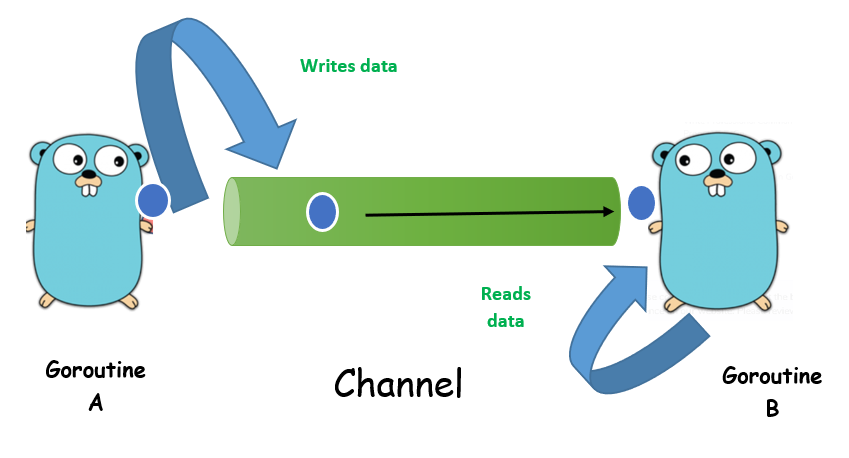
\includegraphics[width=8cm]{sections/gorutine-channel.png}
    \caption{goroutine che comunicano}
    \label{fig:title}
\end{figure}

Cosa significa? In generale i linguaggi come Python, Java, C++ comunicano tramite i thread utilizzando la memoria condivisa, per esempio per accedere ad un array/map/list, e si accede per tutti utilizzando dei lock per garantire la concorrenza, questo Go lo puo fare ma puo anche utilizzare il CSP grazie all'utilizzo di:
\begin{itemize}
    \item goroutine: e' l'unita di esecuzione parallela di Go, simile ai tradizionali thread
    \item channel: struttura concorrente di Go, utilizzata per comunicare tra goroutine diverse
\end{itemize}

\subfile{sections/goroutine}

\subfile{sections/channels}

\subfile{sections/runtimescheduler}

\subfile{sections/utilities}

\end{document}
